\section{Hall Sensors}\label{sec:hallFiltering}

The velocity calculation is made using data from the Hall sensors. There are four magnets on the gear with approximately a quarter of a turn of distance between each. When a magnet passes the hall sensor, a pulse is generated. One way of getting the speed is by calculating the time between two consecutive pulses and relating it to the distance travelled during that time, given by a quarter turn of the drive wheel. A plot of the speed calculated using this method can be seen on \figref{unfilteredHall}.

\begin{figure}[H]
	\centering
	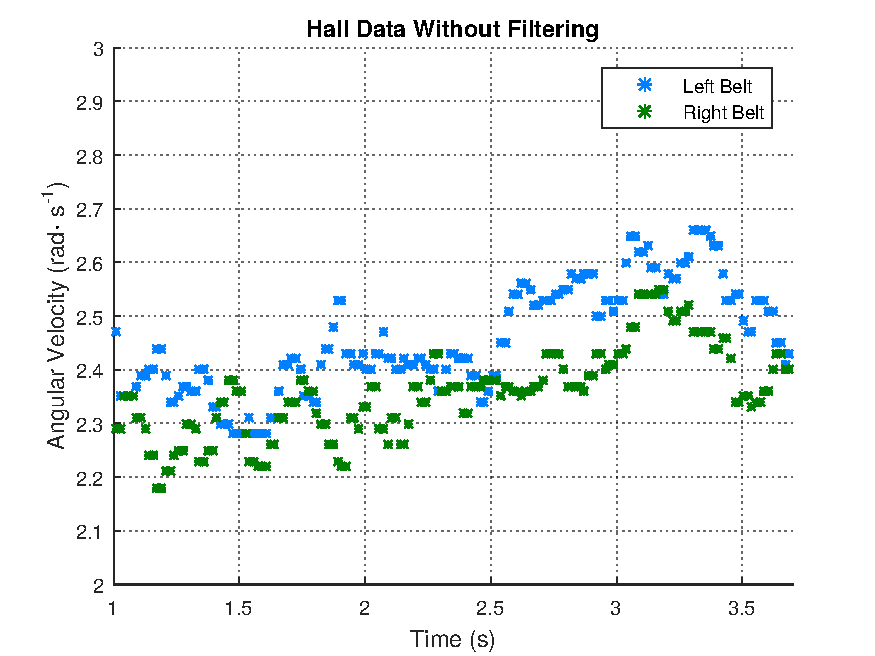
\includegraphics[scale=0.9]{figures/unfilteredHall.pdf}
	\caption{Plot of unfiltered measurements by the Hall sensors}
	\label{unfilteredHall}
\end{figure}


As seen from the graph, this method yields inaccurate measurements due to uneven placement of the magnets. While it might be possible to improve the measurements using filtering, another approach will be tested first.\\

The new approach is to measure the time the wheel takes to make a full turn, to have the exact time and distance of a rotation. The speed will be calculated from a full turn of the drive wheel. Each magnet pulse will then be compared to its own last pass. This means that the first 4 pulses does not yield a speed, since the time of the first rotation happens between the \si{1^{st}} and the \si{5^{th}} pulse. However, the remaining measurements will have the same sampling frequency as the previous. A plot of the measurements using this method can be seen on \figref{filteredHall}.

\begin{figure}[H]
	\centering
	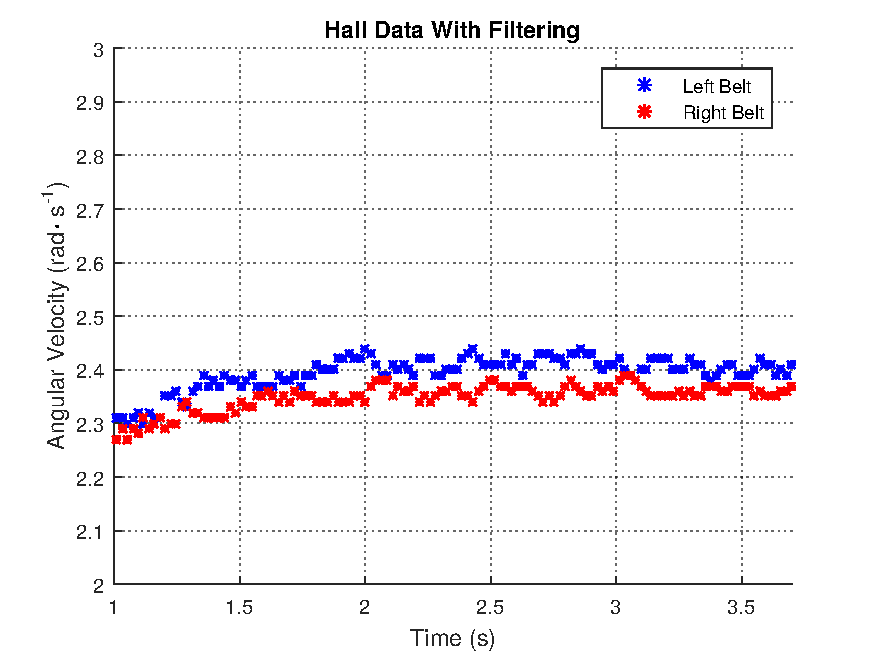
\includegraphics[scale=0.9]{figures/filteredHall.pdf}
	\caption{Plot of filtered measurement by the Hall sensors.}
	\label{filteredHall}
\end{figure}

Comparing \figref{unfilteredHall} and \figref{filteredHall}, the noise has been significantly reduced.
Because of this, filtering will not be necessary, and the new approach using a full turn of the wheel for each measurements is chosen.
% A flowchart of the implementation of the functions of the Hall sensors can be seen on \figref{hallFlowchart}.

% \begin{figure}[H]
% 	\centering
% 	\includegraphics[scale=0.9]{figures/hallFlowchart.pdf}
% 	\caption{Flowchart of the two main functions \textit{tSpeed} and \textit{getSpeed} of the Hall sensors implementation}
% 	\label{hallFlowchart}
% \end{figure}

% This flowchart explains the way of getting the time at each outputs. The Hall sensors use the timers 4 and 5 to register the time of the output. The first function \textit{tSpeed} describes the storing of the two timers values in the registers, the second is a subfunction of the first one, and the last function \textit{getSpeed} is the calculation of the speed from the raw data of a variable in the function \textit{tSpeed}. The two functions \textit{tSpeed} and \textit{getSpeed} are functions of the Hall module.\\


\subsubsection{Minimum Speed}

The Hall sensors measurements can only capture speeds down to a certain value because of the size of the buffer which holds the timer value. The timers can count up to 65 535, and each clock tick lasts 64 µs.\\
A full rotation of the wheel yields a linear movement of \si{166\ mm}, so the minimum measurable speed is given by
%
\begin{flalign}
\eq{\frac{166 \cdot 10^{-3}}{65535 \cdot 64 \cdot 10^{-6}}}	{0,0396}\unit{m \cdot s^{-1}}
\end{flalign}

The Hall Sensors provides data with an acceptable noise level. A filter is therefore not needed for this sensor. The sensors related to the speed have now been explained, and the sensor related to the angle can be described.